\chapter{Grundlagen}
\label{kap2}

\section{Laufroboter}

Dieses Grundlagenkapitel stellt die für diese Arbeit relevanten Laufroboter vor. Dies ist zum einen der \emph{Lauron III}, für den der vorliegende Laufplaner entwickelt wurde; zum anderen ist dies der \emph{Akrobat}, für den der existierende Laufplaner migriert werden soll. Beide sind sich ziemlich ähnlich, jedoch sind die Unterschiede wichtig, um den Laufplaner auf den Akrobat zu migrieren. 

\subsection{Lauron}

Die erste Version des Lauron (Laufender Roboter Neuronal gesteuert) wurde 1994 am Forschungszentrum für Informatik (FZI) in Karlsruhe \autocite{fzi} entwickelt. Zunächst war es das Ziel Laufmuster durch neuronale Netze zu entwickeln und zu testen. Die zweite Version des Lauron verbessert die Sensorausstattung sowie die Mechanik des Laufroboters. Des Weiteren wurde das Steuerungsprinzip, das auf neuronalen Netzen basierte, durch die hierarichische MCA-Architektur \autocite{scholl2001modular} ausgetauscht. Für die dritte Version \emph{Lauron III}, siehe \autoref{kap2:lauron3}, existiert der vorliegende und zu übertragende Laufplaner in Form der 3D-Bibliothek OpenInventor \autocite{inventor}. Daher wird nun näher auf diese Version des Laufroboters sowie auf das grundlegende Konzept des Lauron als Nachahmung der indischen Stabheuschrecke eingegangen. Eine weitere Version des Laufroboters ist der \emph{Lauron IVb}, siehe \autoref{kap2:lauron4b}, welcher sich an der Hochschule Mannheim befindet. Die neuste Version des Laufroboters ist der \emph{Lauron V}.

Der Lauron basiert auf dem Vorbild der indischen Stabheuschrecke (Carausius morosus), die sehr gut erforscht ist. Dies gilt sowohl für den mechanischen Aufbau als auch für die Abläufe der Bewegungen des Roboters. Der Körper ist in drei Teile geteilt.
\begin{itemize}
  \item Kopf (Caput)
  \item Brust (Thorax)
  \item Hinterleib (Abdomen)
\end{itemize}

Die Brust ist wiederum in weitere drei Teile für jeweils ein Beinpaar unterteilt. Damit ergeben sich sechs Beine. Ein Bein besteht aus drei Segmenten:
\begin{itemize}
  \item Hüfte (Coxa)
  \item Oberschenkel (Femur)
  \item Unterschenkel (Tibia)
\end{itemize}

\begin{figure}[b!]
  \centering
  \begin{subfigure}[b]{.4\linewidth}
    \centering
    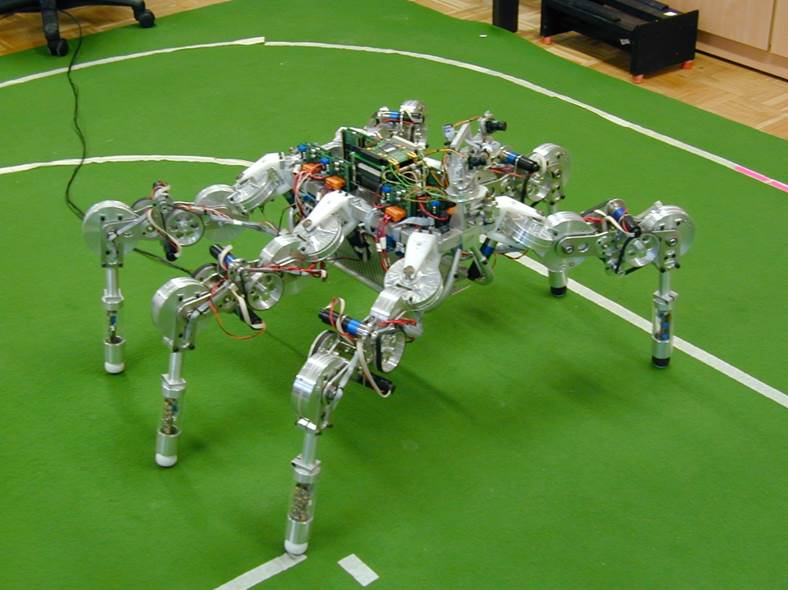
\includegraphics[width=6cm]{kapitel2/lauron3}
    \subcaption{Lauron III}\label{kap2:lauron3}
  \end{subfigure}%
  \qquad
  \begin{subfigure}[b]{.4\linewidth}
    \centering
    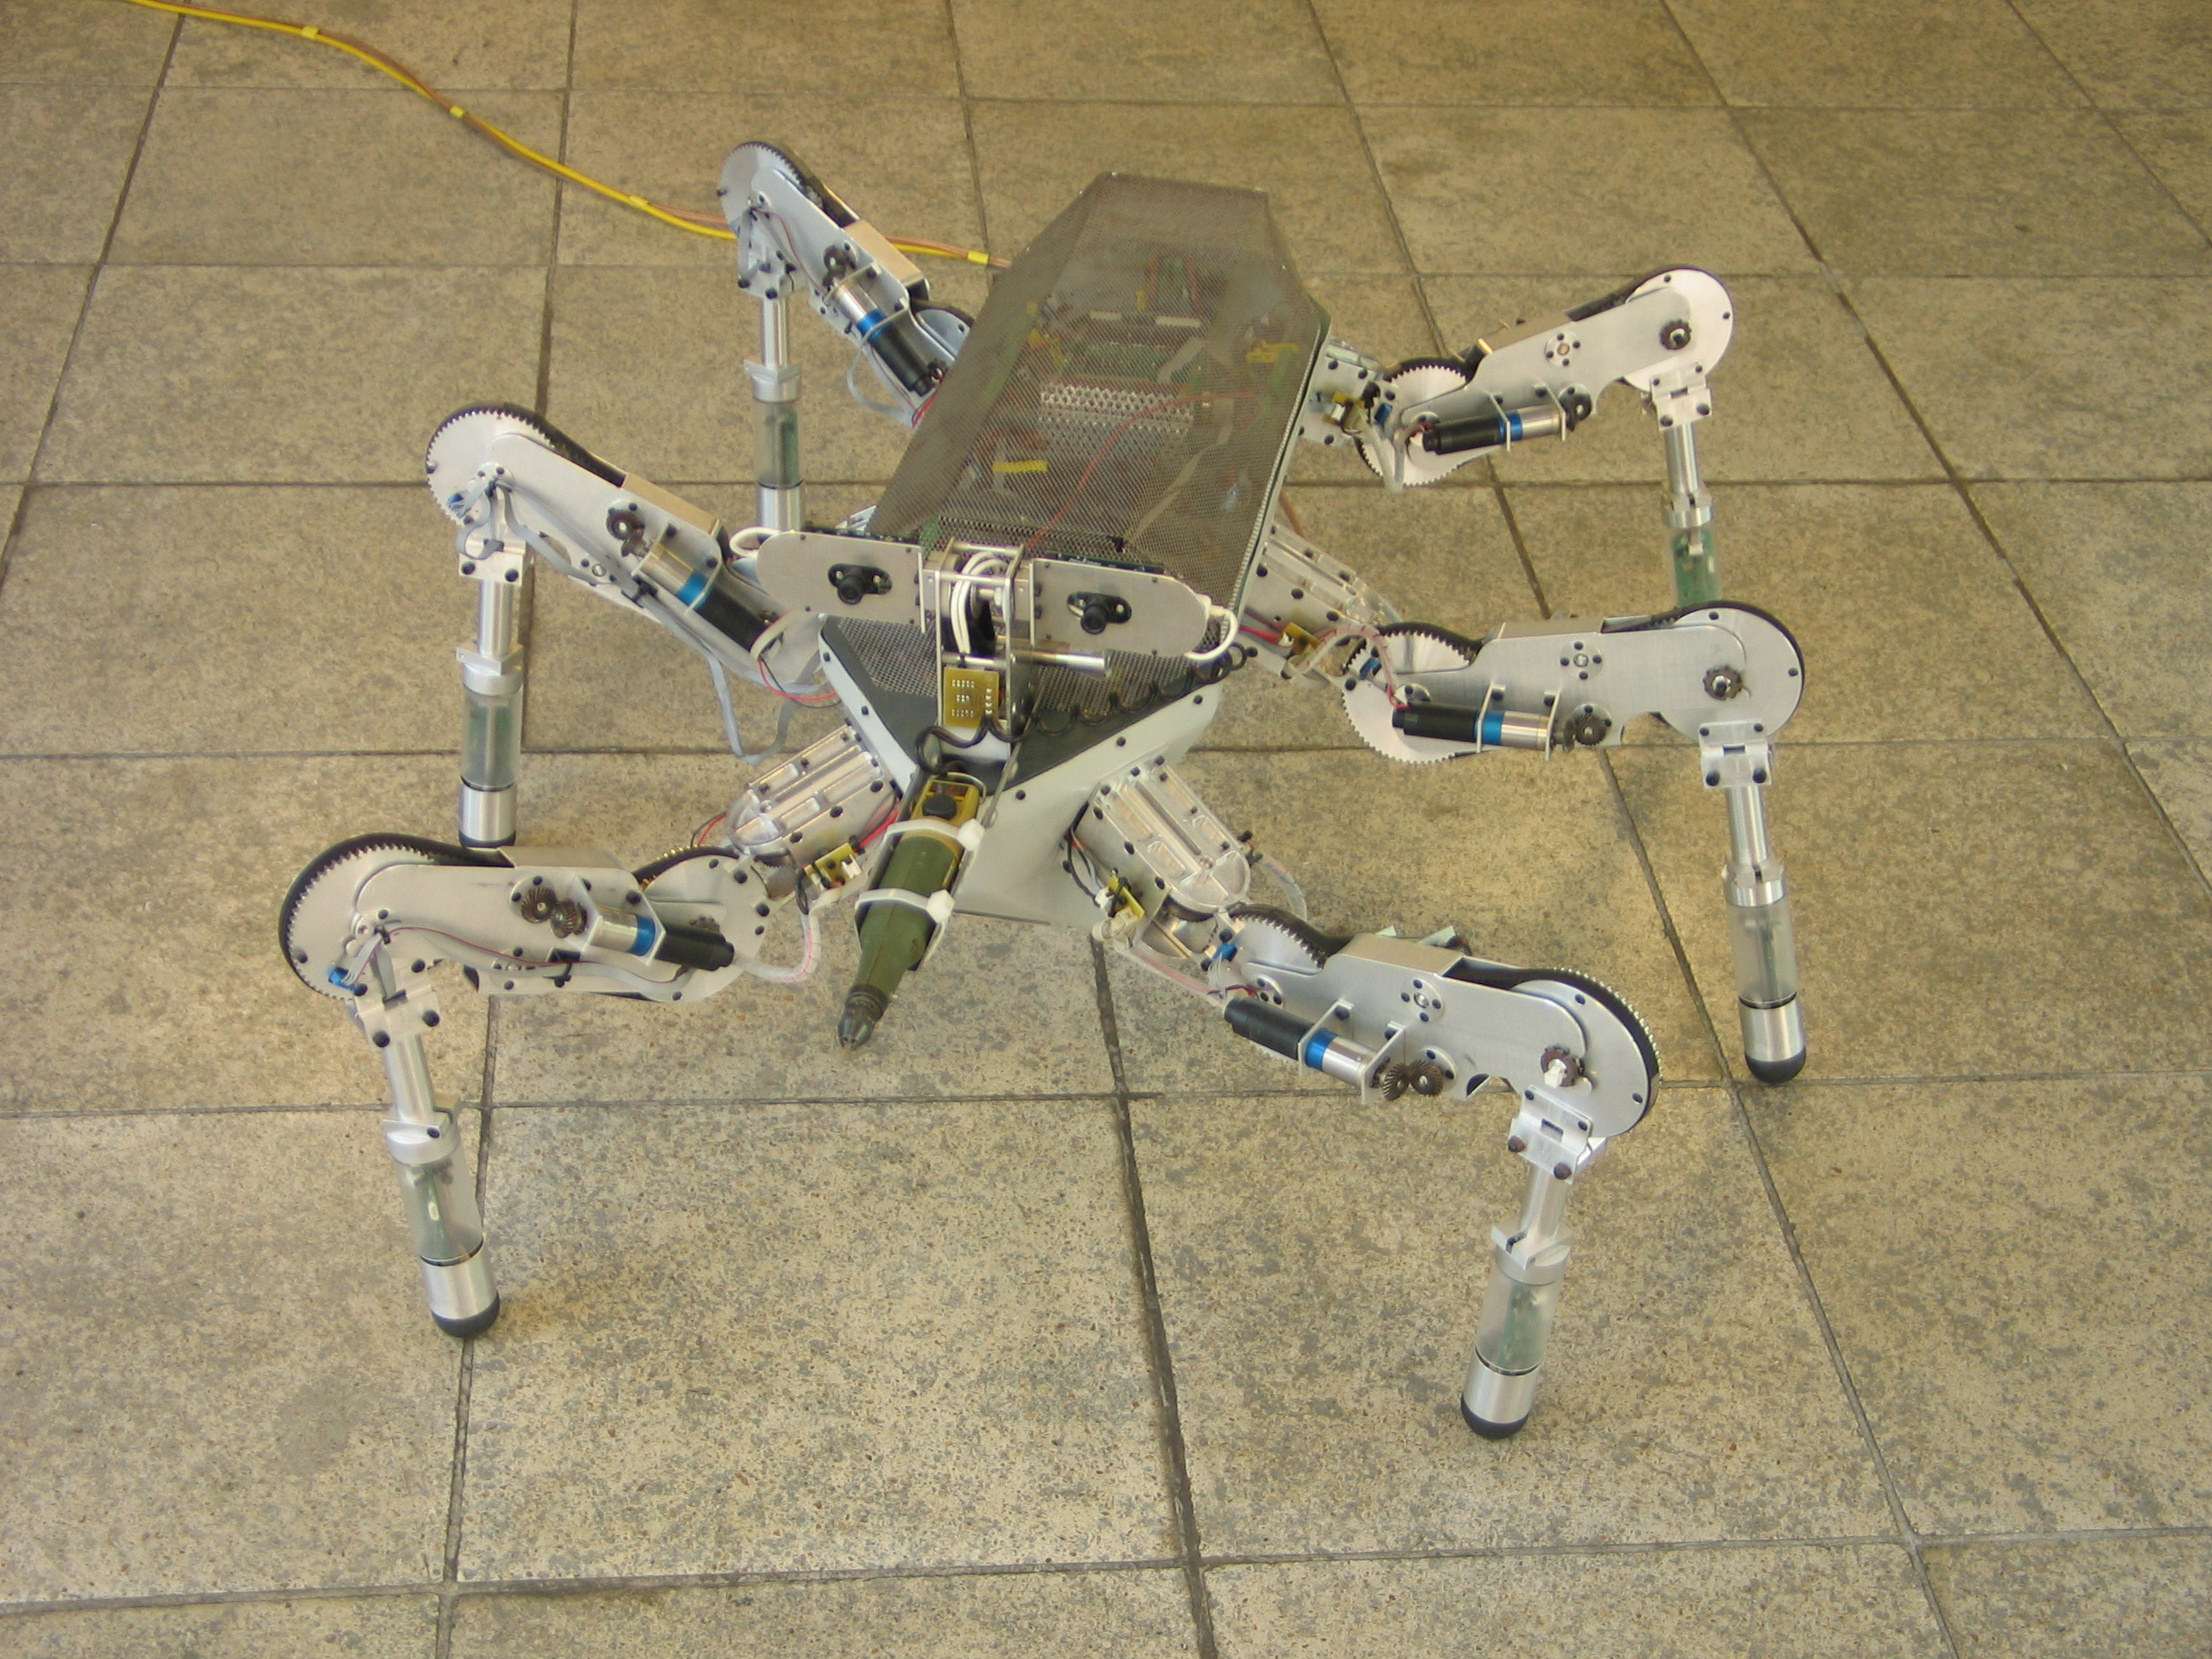
\includegraphics[width=6cm]{kapitel2/lauronivb}
    \subcaption{Lauron IVb}\label{kap2:lauron4b}
  \end{subfigure}\\
  \caption{Verschiedene Versionen des Lauron}
  \label{kap2lauron}
\end{figure}

Die Segmente sind durch die Gelenke Subcoxal $\alpha$, Coxa-Trochanter $\beta$ und Femur-Tibia $\gamma$ verbunden. Der Fuß jedes Beins wird Tarsus genannt. Das erste Gelenk Subcoxal besitzt zwei Freiheitsgrade, die weiteren Gelenke besitzen ein Freiheitsgrad. Damit ist für die indische Stabheuschrecke die minimale erforderliche Zahl an Freiheitsgraden erreicht, damit der Fuß beliebig im dreidimensionalen Raum gesetzt werden kann.

Unter anderem ist noch wichtig, dass der Kopf der indischen Stabheuschrecke zwei lange Fühler besitzt. Diese könnten in einem Roboter beispielsweise als Laserscanner oder Kamera modelliert werden, welche sich einen Überblick über die Gegend verschaffen können.

Der Körper des \emph{Lauron III} trägt die Microcontroller, die Recheneinheit, die Akkumulatoren sowie den Kamerakopf. An beiden Seiten des Körpers sind jeweils drei Beine angebracht. Der Roboter wiegt 16 Kilogramm und hat eine maximale Zuladung von etwa 15kg. Die Maximalgeschwindigkeit beträgt \SI{0.5}{\metre\per\second}. \autocite{gassmann2000} \autocite{troilo2007}

\subsection{Akrobat}

\begin{figure}[b!]
  \centering
  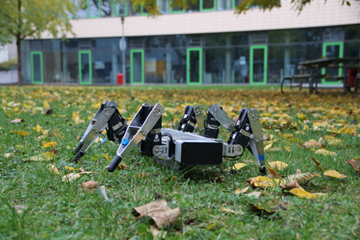
\includegraphics[height=8cm]{kapitel2/akrobat}
  \caption{Der Akrobat vor dem C-Gebäude der Hochschule Mannheim}
  \label{Kap2:akrobat}
\end{figure}

Auch der \emph{Akrobat} (\autoref{Kap2:akrobat}) ist der Form einer Stabheuschrecke nachempfunden und ähnelt in vielerlei Hinsicht dem Lauron.

Der Roboterkörper ist ungefähr 56 Millimeter hoch, 102 Millimeter breit und hat eine Seitenlänge von 62 Millimeter. Ebenfalls besitzt dieser sechs Beine mit je drei Segmenten. Diese haben die Längen 72 Millimeter, 97 Millimeter und 163 Millimeter, welche für kinematische Berechnungen von großer Bedeutung sind. Jedes Bein wiegt ungefähr 0,8 Kilogramm.

Jedes der Gelenke hat exakt einen Freiheitsgrad, sodass das gesamte Bein drei Freiheitsgrade hat. Wie auch beim Lauron ermöglicht dies die beliebige Positionierung im dreidimensionalen Raum. Die Gelenke sind mit dem Servomotor Dynamixel RX64 ausgestattet. Außerdem hat jedes Gelenk einen definierten Arbeitsbereich, welcher nicht unter- oder überschritten werden darf.
\begin{itemize}
  \item $\alpha$: -50$^\circ$ bis 50$^\circ$
  \item $\beta$: -106$^\circ$ bis 106$^\circ$
  \item $\gamma$: -135$^\circ$ bis 135$^\circ$
\end{itemize}  

Außerdem besitzt der Roboter am Kopf eine Kamera, welche aus zwei Freiheitsgraden besteht. Der Roboterkörper verfügt über genügend Freiraum für Batterien im mittleren Gehäuse. Im hinteren Gehäuse ist der Steuerrechner sowie die restliche Elektronik platziert.

Es handelt sich beim Rechner um den Einplatinencomputer Raspberry Pi (Modell B+) mit 521 MB Arbeitsspeicher und einem 700 MHz ARM 11 Prozessor. Der Raspberry Pi bietet vielfältige Anschlussmöglichkeiten: Wireless Local Area Network (WLAN), vier Universal Serial Bus (USB)-Anschlüsse ein Ethernet-Anschluss sowie einen High Definition Multimedia Interface (HDMI)-Anschluss. Über letzteren erfolgt die Visualisierung mittels eines externen Bildschirms. Es besteht die Möglichkeit das Gamepad F710 von Logitech per WLAN anzuschließen. Theoretisch sind auch andere Gamepads möglich, sofern diese im Quellcode konfiguriert wurden. \autocite{askerow2014}

\section{Robotik}

\subsection{Koordinatensysteme}
\subsection{Direkte Kinematik}

- Mit gegebener Stellung der Gelenke Position und Orientierung des Endeffektes zu berechnen
- Transformationsmatrix, die dann aufgelöst wird und berechnet werden kann

fellmann zitieren

\autocite{fellmann2007}

\subsection{Inverse Kinematik}

- Durch Position und Orientierung des Endeffektes mögliche Stellung der Gelenke zu berechnen (meist mehrere Lösungen)
- analytische Berechnung
- numerische Berechnung: lineare Annäherung durch Jacobi-Matrix

fellmann zitieren

\autocite{fellmann2007}

\subsection{Laufplanung}

statische Laufalgorithmen, reaktive, planende Laufalgorithmen like RandomSampling

\section{Frameworks}

\subsection{Robot Operating System}
\subsection{Gazebo}
\subsection{MeshLab}